\documentclass[10pt]{article}

\usepackage[margin=1in]{geometry}
\usepackage{amsmath}
\usepackage{amssymb}
\usepackage{amsthm}
\usepackage{mathtools}
\usepackage{bm}

\usepackage{color}
\usepackage{colortbl}
\definecolor{deepblue}{rgb}{0,0,0.5}
\definecolor{deepred}{rgb}{0.6,0,0}
\definecolor{deepgreen}{rgb}{0,0.5,0}
\definecolor{gray}{rgb}{0.7,0.7,0.7}

\usepackage{hyperref}
\hypersetup{
  colorlinks   = true, %Colours links instead of ugly boxes
  urlcolor     = black, %Colour for external hyperlinks
  linkcolor    = blue, %Colour of internal links
  citecolor    = blue  %Colour of citations
}

%%%%%%%%%%%%%%%%%%%%%%%%%%%%%%%%%%%%%%%%%%%%%%%%%%%%%%%%%%%%%%%%%%%%%%%%%%%%%%%%

\theoremstyle{definition}
\newtheorem{advanced}{Optional Advanced Problem}
\newtheorem{problem}{Problem}
\newtheorem{note}{Note}
\newtheorem{defn}{Definition}
\newtheorem{example}{Example}
\newcommand{\E}{\mathbb E}
\newcommand{\R}{\mathbb R}
\DeclareMathOperator{\nnz}{nnz}
\DeclareMathOperator{\determinant}{det}
\DeclareMathOperator{\Var}{Var}
\DeclareMathOperator{\rank}{rank}
\DeclareMathOperator*{\argmin}{arg\,min}
\DeclareMathOperator*{\argmax}{arg\,max}

\newcommand{\I}{\mathbf I}
\newcommand{\Q}{\mathbf Q}
\newcommand{\p}{\mathbf P}
\newcommand{\pb}{\bar {\p}}
\newcommand{\pbb}{\bar {\pb}}
\newcommand{\pr}{\bm \pi}

\newcommand{\trans}[1]{{#1}^{T}}
\newcommand{\loss}{\ell}
\newcommand{\w}{\mathbf w}
\newcommand{\x}{\mathbf x}
\newcommand{\y}{\mathbf y}
\newcommand{\lone}[1]{{\lVert {#1} \rVert}_1}
\newcommand{\ltwo}[1]{{\lVert {#1} \rVert}_2}
\newcommand{\lp}[1]{{\lVert {#1} \rVert}_p}
\newcommand{\linf}[1]{{\lVert {#1} \rVert}_\infty}
\newcommand{\lF}[1]{{\lVert {#1} \rVert}_F}

%%%%%%%%%%%%%%%%%%%%%%%%%%%%%%%%%%%%%%%%%%%%%%%%%%%%%%%%%%%%%%%%%%%%%%%%%%%%%%%%

\begin{document}


\begin{center}
{
\Huge
Notes: Computational Linear Algebra
}

\vspace{0.15in}
%Due: Sunday, 30 Aug 2020 by midnight
\end{center}

\begin{center}
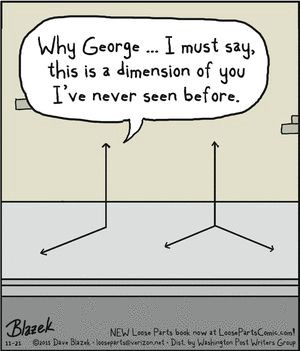
\includegraphics[height=1.8in]{comic}
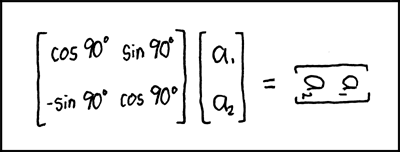
\includegraphics[height=1.8in]{matrix_transform}
\end{center}

%%%%%%%%%%%%%%%%%%%%%%%%%%%%%%%%%%%%%%%%

\section{Introduction}

This set of notes covers how to compute the runtimes of linear algebra expressions similar to
\begin{equation}
\lF{(\lambda I + A) \x \trans \x}
.
\end{equation}
We will be doing these calculations many times throughout the course,
and so it is necessary to master this material to get a passing grade.

\begin{note}
If you find any errors in these notes (or any other class material),
you can get extra credit by submitting a pull request to github fixing the error.
\end{note}

%\section{Linear Algebra Review}

\begin{note}
Many students struggle in this course with basic linear algebra concepts like the rank of a matrix and eigenvalues.
If you would like more background on these topics, I recommend watching the 3blue1brown videos on linear algebra:
\begin{quote}
    \url{https://www.3blue1brown.com/essence-of-linear-algebra-page}
\end{quote}
\end{note}

\section{Big-O/$\Theta$/$\Omega$ Notation}

You are likely familiar with asymptotic notation from your data structures class,
where you used it to measure the time and space complexity of algorithms.
In this class,
we will also be measuring statistical complexity of algorithms.
The statistical complexity will result in formulas a bit more complex than you have likely seen before,
and so you will need to be intimately familiar with the formal definitions of asymptotic notation.
There are many equivalent definitions, but in this class, we will use the following.

\begin{defn}
    Let $f,g$ be (possibly multivariate) functions from $(\R^+)^d\to\R^+$,
    where $d>0$ is an integer that specifies the number of input variables.
    Then,
    \begin{enumerate}
        \item If $\displaystyle\lim_{\x\to\infty} \frac{f(\x)}{g(\x)} < \infty$, then we say $f = O(g)$.
        \item If $\displaystyle\lim_{\x\to\infty} \frac{f(\x)}{g(\x)} > 0$, then we say $f = \Omega(g)$.
        %\item If $\lim_{x\to\infty} \frac{f(x)}{g(x)} = 0$, then we say $f = O(g)$.
        \item We say that $f = \Theta(g)$ if both $f=O(g)$ and $f=\Omega(g)$.
    \end{enumerate}
    Intuitively, you should think of $O$ as $\le$, $\Omega$ as $\ge$, and $\Theta$ as $=$.
\end{defn}



\newpage
\begin{note}
You are not required to complete and submit the problems in this packet,
but the problems on the quizzes/exams will be very similar,
so I strongly recommend you complete all of these problems.
\end{note}

\begin{problem}
    Complete each equation below by adding the symbol $O$ if $f=O(g)$, $\Omega$ if $f=\Omega(g)$, or $\Theta$ if $f=\Theta(g)$.  
    The first row is completed for you as an example.

{\renewcommand{\arraystretch}{4.4}
\begin{tabular}{c c c c c c}
    & f(n) &~\hspace{0.5in}~$ $~\hspace{0.5in}~& g(n) &\\
    \hline
    & $1$ & ~\hspace{0.5in}~$=$~\hspace{0.5in}~  & $O(n)$ &  &\\
    \arrayrulecolor{gray}\hline
    & $3 n\log n$ & ~\hspace{0.5in}~$=$~\hspace{0.5in}~  & $n^2$ &  &\\
    \arrayrulecolor{gray}\hline
    & $1$ & ~\hspace{0.5in}~$=$~\hspace{0.5in}~  & $1/n$ &  &\\
    \arrayrulecolor{gray}\hline
    & $\log_2 n$ & ~\hspace{0.5in}~$=$~\hspace{0.5in}~  & $\log_3 n$ &  &\\
    \arrayrulecolor{gray}\hline
    & $\log n$ & ~\hspace{0.5in}~$=$~\hspace{0.5in}~  & $\frac {1} {\log n}$ &  &\\
    \arrayrulecolor{gray}\hline
    & $5\cdot10^{30}$ & ~\hspace{0.5in}~$=$~\hspace{0.5in}~  & $\log n$ &  &\\
    \arrayrulecolor{gray}\hline
    & $\log n$ & ~\hspace{0.5in}~$=$~\hspace{0.5in}~  & $\log (n^2)$ &  &\\
    \arrayrulecolor{gray}\hline
    & $2^n$ & ~\hspace{0.5in}~$=$~\hspace{0.5in}~  & $3^n$ &  &\\
    \arrayrulecolor{gray}\hline
    & $\frac 1 n$ & ~\hspace{0.5in}~$=$~\hspace{0.5in}~  & $\sqrt{\frac 1 n}$ &  &\\
    \arrayrulecolor{gray}\hline
    & $\log n$ & ~\hspace{0.5in}~$=$~\hspace{0.5in}~  & $(\log n)^2$ &  &\\
    \arrayrulecolor{gray}\hline

    %& $O(1)$ & or & $O(n)$ & or & equal\\
    %& $O(n\log n)$ & or & $O(n^2)$ & or & equal\\
    %& $\Theta(1)$ & or & $\Theta(1/n)$ & or & equal\\
    %& $\Omega(\log_2 n)$ & or & $\Omega(\log_3 n)$ & or & equal\\
    %& $O(n^{42})$ & or & $O(42^n)$ & or & equal\\
    %& $\Theta(5\cdot10^{30})$ & or & $\Theta(\log n)$ & or & equal\\
    %& $\Omega(\log n)$ & or & $\Omega(\log (n^2))$ & or & equal\\
    %& $O(2^n)$ & or & $O(3^n)$ & or & equal\\
    %& $\Theta(n!)$ & or & $\Theta(n^2)$ & or & equal\\
    %& $\Omega(\log n)$ & or & $\Omega((\log n)^2)$ & or & equal\\
\end{tabular}
}
\end{problem}

\newpage
\begin{problem}
    Complete each equation below by adding the symbol $O$ if $f=O(g)$, $\Omega$ if $f=\Omega(g)$, or $\Theta$ if $f=\Theta(g)$.  
    If $f$ cannot be related to $g$ using asymptotic notation, draw a slash through the equals sign.
    The first row is completed for you as an example.

{\renewcommand{\arraystretch}{4.4}
\begin{tabular}{c c c c c c}
    & f(a,b,c) &~\hspace{0.5in}~$ $~\hspace{0.5in}~& g(a,b,c) &\\
    \hline
    & $ab$ & ~\hspace{0.5in}~$=$~\hspace{0.5in}~  & $\Omega(b)$ &  &\\
    \arrayrulecolor{gray}\hline
    & $a + b$ & ~\hspace{0.5in}~$=$~\hspace{0.5in}~  & $ab$ &  &\\
    \arrayrulecolor{gray}\hline
    & $a^2b$ & ~\hspace{0.5in}~$=$~\hspace{0.5in}~  & $ab^2$ &  &\\
    \arrayrulecolor{gray}\hline
    & $a\log b$ & ~\hspace{0.5in}~$=$~\hspace{0.5in}~  & $a \log^2 b$ &  &\\
    \arrayrulecolor{gray}\hline
    & $a^2bc^3$ & ~\hspace{0.5in}~$=$~\hspace{0.5in}~  & $a^2b^2c^3$ &  &\\
    \arrayrulecolor{gray}\hline
    & $\frac ab$ & ~\hspace{0.5in}~$=$~\hspace{0.5in}~  & $\frac a {b^2}$ &  &\\
    \arrayrulecolor{gray}\hline
    & $\frac ab$ & ~\hspace{0.5in}~$=$~\hspace{0.5in}~  & $(\frac a b)^2$ &  &\\
    \arrayrulecolor{gray}\hline
    & $\frac{ab}{c}$ & ~\hspace{0.5in}~$=$~\hspace{0.5in}~  & $\frac{a}{c}$ &  &\\
    \arrayrulecolor{gray}\hline
    & $\frac{a}{bc}$ & ~\hspace{0.5in}~$=$~\hspace{0.5in}~  & $\frac{a}{c^2}$ &  &\\
    \arrayrulecolor{gray}\hline
    & $\frac{a+b+c}{c}$ & ~\hspace{0.5in}~$=$~\hspace{0.5in}~  & $\frac{a+b}{c}$ &  &\\
    \arrayrulecolor{gray}\hline

    %& $O(1)$ & or & $O(n)$ & or & equal\\
    %& $O(n\log n)$ & or & $O(n^2)$ & or & equal\\
    %& $\Theta(1)$ & or & $\Theta(1/n)$ & or & equal\\
    %& $\Omega(\log_2 n)$ & or & $\Omega(\log_3 n)$ & or & equal\\
    %& $O(n^{42})$ & or & $O(42^n)$ & or & equal\\
    %& $\Theta(5\cdot10^{30})$ & or & $\Theta(\log n)$ & or & equal\\
    %& $\Omega(\log n)$ & or & $\Omega(\log (n^2))$ & or & equal\\
    %& $O(2^n)$ & or & $O(3^n)$ & or & equal\\
    %& $\Theta(n!)$ & or & $\Theta(n^2)$ & or & equal\\
    %& $\Omega(\log n)$ & or & $\Omega((\log n)^2)$ & or & equal\\
\end{tabular}
}
\end{problem}

%\newpage
%\begin{problem}
    %Prove or provide a counter example.
    %For any two (possibly multivariate) functions $f$ and $g$,
    %at least one of the following must be true:
    %\begin{enumerate}
        %\item $f = O(g)$,
        %\item $g = O(f)$.
    %\end{enumerate}
%\end{problem}

\newpage
\begin{note}
The main advantage of asymptotic notation is that it lets us write complex formulas in simpler forms,
focusing only on the ``most important'' parts.
\end{note}
\begin{problem}
    Simplify the following expressions:

\begin{enumerate}
    \item $O\bigg(n^3 + 5n^2\log n + \log n \bigg)$
    \vspace{1.5in}
\item $O\bigg(ab^2 + 3a^2b + ab + 10b\bigg)$
    \vspace{1.5in}
\item $O\bigg(a + b + c + ab + bc + abc\bigg)$
    \vspace{1.5in}
\item $O\bigg(\frac 1 n + \frac 1 {n^2}\bigg)$
    \vspace{1.5in}
\item $O\bigg(\frac 1 n + \frac 1 {nm} + \frac 1 m \bigg)$
    \vspace{1.5in}
%\item $\Omega\bigg((3.45n + n)(\log n^2)\bigg)$
    %\vspace{1.5in}
%\item $\Theta\bigg(n(1 + \log n) + n^{3.2} + \log 2^n\bigg)$
    %\vspace{1.5in}
\end{enumerate}
\end{problem}

%%%%%%%%%%%%%%%%%%%%%%%%%%%%%%%%%%%%%%%%

\newpage
\section{BLAS}

The \emph{Basic Linear Algebra Subprogram} (BLAS) is a standard interface for simple vector and matrix operations.
BLAS libraries are written in low-level languages like Assembly, C, Fortran, and CUDA.
PyTorch provides an ``easy to use'' interface to these BLAS operations.
We will gloss over many technical details in these notes and focus on high-level asymptotic runtimes.

\subsection{Notation}

We will typically use capital letters $(A, B, C)$ to denote matrices,
bold lower case letters $(\textbf x, \textbf y, \textbf z)$ to denote vectors,
and lower case italics letters $(n, m, o)$ to denote scalars.

\subsection{Dense vs Sparse Matrices}

Mathematicians define a \emph{sparse matrix} to be any matrix with a large number of zero entries relative to the total number of entries,
and a \emph{dense matrix} to be any matrix with few zeros.
There is no strict cut-off here, but it's typical for a sparse matrix to have $< 1\%$ of its entries be zero.
We will use the function $\nnz(A)$ to represent the total \emph{Number of Non Zero} values of the matrix $A:\R^{m\times n}$.

\begin{problem}
What is the $\nnz$ of the following matrices?

%\begin{enumerate}
    %\item
\begin{align*}
    A &= \begin{pmatrix} 0 & 1 & 0 \\ 0 & 0 & 0 \\ -1 & 0 & 0 \end{pmatrix} & \nnz(A) = \\
        \\
    B &= \begin{pmatrix} 1 & 2 \\ 3 & 4 \\ 5 & 6 \end{pmatrix} & \nnz(B) = \\
        \\
    C &= \begin{pmatrix} 0.0 & 0.1 & 0.2 \\ 0.3 & 0.4 & 0.5 \end{pmatrix} & \nnz(C) = \\
\end{align*}
%\end{enumerate}

\end{problem}
\vspace{4in}

%There are many data structures for storing sparse matrices.
%These include:
%\begin{enumerate}
    %\item Dictionary of keys (DOK),
    %\item List of lists (LIL),
    %\item Coordinate list (COO),
    %\item Compressed sparse row (CSR, CRS or Yale format), and
    %\item Compressed sparse column (CSC or CCS).
%\end{enumerate}
%In this class, we will not cover the details of the different formats.
%Pytorch implements both the COO and CSR formats,
%and you are responsible for understanding when to use each of these formats.\footnote{
    %The documentation is at \url{https://pytorch.org/docs/stable/sparse.html}.
%}
%From here on out the notes always assume that a sparse matrix is stored in either COO or CSR format.
\begin{problem}
    Describe data structures optimized for sparse and dense matrices.
\end{problem}

\newpage
\subsection{Memory Usage}

If $A$ is stored as a sparse matrix,
the memory usage is $\Theta(\nnz(A))$.
If $A$ is stored as a dense matrix,
the memory usage is $\Theta(mn)$.

\begin{problem}
    Prove or provide a counter example.
    For both sparse and dense matrices,
    the storage requirements are $O(mn)$.
    \vspace{4in}
\end{problem}

\newpage
\begin{note}
    You must be able to perform basic calculations about the exact amount of memory we expect dense matrices to consume.
    For sparse matrices, you are only responsible for the asymptotic calculations.
\end{note}
\begin{problem}
    A computer has 8GB of RAM.
    What is the largest dense vector of 64bit floating point numbers that can fit in memory?
    \vspace{4in}
\end{problem}

\begin{problem}
    You have a dataset with $2^{10}$ columns and $2^{20}$ rows.
    It is stored using 16bit floating point numbers.
    How much memory does this dataset consume?
    \vspace{4in}
\end{problem}

\newpage
\subsection{BLAS Level 1}

BLAS Level 1 routines are for linear algebra operations that only involve vectors.
These include the dot product, vector norms, addition, and scalar multiplication.

These are fully implemented in PyTorch for both sparse and dense vectors.
For dense vectors of length $n$, the runtime of all operations is $\Theta(n)$.
For sparse vectors, all operations of a single vector $\x$ take time $\Theta(\nnz(\x))$
and all operations of two vectors $\x$ and $\y$ take time $\Theta(\nnz(\x)+\nnz(\y))$.

\begin{problem}
    What is the runtime of the following expressions?
    You should report the answer for every possible combination of sparse/dense vectors.
    \begin{enumerate}
        \item $5 \cdot \x$
            \vspace{2in}
        \item $0 \cdot \x$
            \vspace{2in}
        \item $\trans\x \y$
            \vspace{2in}
        \item $\lone{\x}$
            \vspace{2in}
    \end{enumerate}
\end{problem}

\begin{problem}
    What is the formula for the following vector norms?
    What is the runtime for computing these formula in both the sparse and dense case?
    \begin{enumerate}
        \item $\lone{\x}=$
            \vspace{2in}
        \item $\ltwo{\x}=$
            \vspace{2in}
        \item $\linf{\x}=$
            \vspace{2in}
        %\item $\lp{\x}=$
            %\vspace{2in}
    \end{enumerate}
\end{problem}

\newpage
\subsection{BLAS Level 2}

BLAS Level 2 routines are for vector-matrix operations.
The main examples are the products $A\x$ and $\x A$.
%PyTorch fully supports these operations in dense matrices,
%but has only partial support in sparse matrices.
%The sparse matrix support is via BLAS Level 3,
%so we will only discuss that.
Up to constant factors, these operations have the same run times as the BLAS level 3 operations, so we will only discuss the level 3 operations below.

\subsection{BLAS Level 3}

BLAS Level 3 routines are for matrix-matrix operations.
Let $A : \R^{m\times n}$ and $B : \R^{n \times o}$.
Note that when $o=1$, then $B$ is a vector, and so BLAS Level 3 operations can be used to implement BLAS Level 2 operations.

For dense matrices, matrix multiplication $AB$ takes time $O(mno)$.
This is often referred to as a ``cubic'' runtime because when the multiplied matrices are square,
and thus $m=n=o$,
the runtime is $O(n^3)$.
There are good algorithms that take potentially much less time than this,
with the best known taking time $O(n^{2.371552})$.
No BLAS implementation that I know of actually implements this algorithm due to the very high constant factor,
and Strassen's algorithm with runtime $\Theta(n^{\log_2 7})\approx\Theta(n^{2.807})$ is the most commonly used algorithm.
Currently, we know that matrix multiplication takes at least time $\Omega(n^2\log n)$,
and it is an open problem what the optimal runtime for matrix multiplication is.
The following wikipedia link has more details:
\begin{quote}
    \url{https://en.wikipedia.org/wiki/Computational_complexity_of_matrix_multiplication}
\end{quote}

For sparse matrices, PyTorch has only limited support for BLAS Level 2/3.
In particular, PyTorch allows the first matrix to be either sparse or dense,
but the second matrix must be dense.
The runtime in the sparse case is $\Theta(\nnz(A)o)$.
The output is always a dense tensor.

The runtime of computing the transpose is $\Theta(1)$
for both sparse and dense matrices.
Libraries do not actually do any computation when you call a transpose function.
They just store a flag that the matrix has been transposed;
then, when performing a mathematical operation, the memory is read in the transposed order.

The runtime of addition and scalar multiplication is linear in the memory usage of the affected matrices.

\begin{note}
For the following problems, always assume that the dimensions match so that the expressions are well defined.
You will have to specify the dimensions.
\end{note}

\begin{problem}
    What is the runtime of the following expressions?
    You should report the answer for every possible combination of sparse/dense matrices.

    \begin{enumerate}
        \item
            $A + B$
            \vspace{1.5in}
        \item
            $A + \trans B$
            \vspace{1.5in}
        \item
            $3A$
            \vspace{1.5in}
        \item
            $AB$
            \vspace{1.5in}
        \item
            $A\trans B$
            \vspace{1.5in}
        \item
            $A\x$
            \vspace{1.5in}
        \item
            $\x A$
            \vspace{1.5in}
    \end{enumerate}
\end{problem}

%\begin{problem}
    %What is the runtime of the following expressions?
    %You should report the answer for every possible combination of sparse/dense matrices.
    %\begin{enumerate}
        %\item
            %$\trans B \trans A$
            %\vspace{1in}
        %\item
            %$\trans \x \x$
            %\vspace{1in}
        %\item
            %$\x\trans \x$
            %\vspace{1in}
        %\item
            %$A\x + \x$
            %\vspace{1in}
        %\item
            %$(A+I)\x$
            %\vspace{1in}
    %\end{enumerate}
%\end{problem}

\newpage
\begin{problem}
    Let $A$ be a sparse matrix, and $B$ be a dense matrix.
        Then the matrix product $AB$ can be computed directly in PyTorch,
        but the matrix product $BA$ cannot be computed directly because the first matrix is not sparse.
        It is nevertheless still possible to compute $BA$ by rewriting the expression so that a sparse matrix appears on the left hand side of a matrix multiplication.
        How?
\end{problem}
\vspace{4in}

\begin{problem}
    Recall that in PyTorch---and many other linear algebra libraries---only the first matrix in a matrix multiplication can be sparse,
    and the second must be dense.
    The reason is that the sparsity of the matrix product $AB$ is impossible to predict from the sparsity of just $A$ and $B$.

    In this problem, you will prove this fact by example.
    Your task is to construct a family of $m\times m$ matrices $A$ and $B$ such that
    \begin{equation}
        \nnz(AB) = O(1)
        \qquad
        \text{and}
        \qquad
        %\nnz(\trans B \trans A) = O(mno)
        \nnz(BA) = \Omega(m^2)
        .
    \end{equation}
    \vspace{3in}
\end{problem}

%\newpage
%\begin{note}
    %Strassen's algorithm is a famous divide and conquer algorithm for fast matrix multiplication.
    %It is the most commonly implemented algorithm in BLAS libraries because it has both good constant factors and good asymptotic performance.
    %Lookup this algorithm and understand why it works.
    %This is a problem that every computer science undergrad should do at some point in their undergrad career.
%\end{note}


%%%%%%%%%%%%%%%%%%%%%%%%%%%%%%%%%%%%%%%%

\newpage
\subsection{Matrix Chain Ordering Problem (MCOP)}

Matrix multiplication is famously not commutative, but it is associative.
That is, no matter where you place the parentheses,
you will get the same answer.
Computationally, however, some choices of parentheses can be much better than others.

\begin{problem}
    Let $A : \R^{m\times n}$, $B : \R^{n\times o}$, $C : \R^{o\times p}$.

    \begin{enumerate}
        \item What is the runtime of computing $(AB)C$?
            \vspace{2in}
        \item What is the runtime of computing $A(BC)$?
            \vspace{2in}
        \item Under what conditions would you choose the former parenthesization over the latter?
            \vspace{2in}
    \end{enumerate}
\end{problem}

\newpage

\begin{problem}
Recall that in PyTorch---and many other linear algebra libraries---only the first matrix in a matrix multiplication can be sparse,
and the second must be dense.

Let $A$ and $C$ be sparse matrices, and $B$ be a dense matrix.
How can we compute the product $ABC$?\footnote{
Hint: You can swap the order of matrix multiplications by using the fact that for any two matrices $X$ and $Y$, $XY = \trans{(\trans Y \trans X)}$.
    }
\end{problem}

\newpage
\begin{note}
The \emph{Matrix Chain Ordering Problem} (MCOP) is the problem of finding the optimal ordering of parentheses for a given sequence of $n$ matrices.
There is a classic dynamic programming solution to this problem that takes time $\Theta(n^3)$.
%\footnote{It's important to note that the $n$ here refers to the number of matrices, not the dimensions of any given matrices.}
(It's important to note that the $n$ here refers to the number of matrices, not the dimensions of any given matrices.)
Many more complicated algorithms exist for solving MCOP,
the best of which currently takes time $\Theta(n \log n)$.
The best known lower bound for MCOP is $\Omega(n)$,
and it is therefore an open problem whether MCOP can be solved in linear time.
%\end{note}

%\begin{note}
The $\Theta$ and $\Omega$ notation above is correct.
It should be ``obvious''\footnote{In mathematics, the word \emph{obvious} has a different meaning than ordinary English.  In mathematics, it means that the claim follows directly from the definitions.  It still might take you 20-30 minutes of thinking about the definitions to verify the claim, however.} why these values are consistent with each other and do not contradict the definitions of $\Theta$ and $\Omega$.
\end{note}

%\begin{problem}
    %(Optional)
    %Give the dynamic programming solution for MCOP.
    %This is a problem that every computer science undergrad should do at some point in their undergrad career.
%\end{problem}

\begin{problem}
    \label{prob:8}
    Parenthesization becomes critical when the matrices are vectors.
    What is the optimal way to parenthesize the expressions:
    \begin{enumerate}
        \item
            $\trans \x \x \trans \x \x$?
            \vspace{3in}
        \item
            $\x \trans \x \x \trans \x$?
            \vspace{3in}
    \end{enumerate}
\end{problem}

\begin{problem}
    Based on your solution to Problem \ref{prob:8} above,
    what is the asymptotically fastest way to compute the following expression
    \begin{equation}
        \prod_{i=1}^n (\x \trans \x)
    \end{equation}
    \vspace{2in}
\end{problem}

%%%%%%%%%%%%%%%%%%%%%%%%%%%%%%%%%%%%%%%%

\newpage
\section{Beyond BLAS}

Let $A : \R^{n \times n}$.
The matrix inverse $A^{-1}$ and matrix determinant $\determinant(A)$ can both be computed in time $O(n^3)$.
There are asymptotically faster algorithms for computing these runtimes,
but they are less important than the matrix multiplication algorithms.
The runtime of computing the top-$k$ eigenvectors and eigenvalues is $O(kn^2)$.%
\footnote{
In the next set of notes, we will see that the pagerank technique is equivalent to computing the top eigenvalue of a matrix.
We will then explore several algorithms for computing eigenvalues that have faster but more complex runtime expressions.
For this set of notes, however, just assume that computing the top-$k$ eigenvectors takes time $O(kn^2)$ as stated above.
}

For each of these operations, PyTorch has full support for dense matrices,
but no support for sparse matrices.

%\begin{problem}
    %Let $\x : \R^n$
    %and 
    %$A : \R^{n\times n}$.
    %What is the formula for the following matrix norms?
    %(Note that the $\ltwo{\cdot}$ and $\lp{\cdot}$ norms are defined differently for matrices than vectors.)
    %\begin{enumerate}
        %\item $\ltwo{A}$
            %\vspace{2in}
        %\item $\lp{A}$
            %\vspace{2in}
        %\item $\lF{A}$
            %\vspace{2in}
    %\end{enumerate}
%\end{problem}
%
%\newpage
%\begin{problem}
    %Use the formulas above to calculate the runtime of computing the following matrix norms.
    %\begin{enumerate}
        %\item $\ltwo{A}$
            %\vspace{4in}
        %\item $\lF{A}$
            %\vspace{4in}
    %\end{enumerate}
    %We do not have enough tools yet for calculating the runtime of generic $\lp{\cdot}$ norms,
    %and that's why I didn't ask you to provide that runtime.
%\end{problem}
%
%\newpage
\begin{problem}
    Let $A : \R^{m \times n}$, $\x : \R^n$, and $\lambda : \R$.
    Assume that $A$ and $\x$ are dense.
    What is the runtime for computing the following expressions?
    \begin{enumerate}
        \item $A^{-1}\x$
            \vspace{4in}
            \newpage
        \item $(A \trans A)^{-1} A \x$
            \vspace{4in}
            \newpage
        \item $A (\trans A A)^{-1}$
            \vspace{4in}
            \newpage
        \item $\lF{A \trans A A \x}^2$
            \vspace{4in}
            \newpage
        \item $\lF{(\lambda I + A) \x \trans \x}$

            Note that $I$ is the identity matrix.
            For the expression above to be well defined, $m$ must be equal to $n$.
            \vspace{4in}
    \end{enumerate}
\end{problem}

%%%%%%%%%%%%%%%%%%%%%%%%%%%%%%%%%%%%%%%%

%\subsection{(Optional) Tensors}
%
%Tensors are higher order versions of vectors and matrices,
%and PyTorch is designed to handle tensors efficiently.
%There are many open problems related to computing tensor operations efficiently,
%but PyTorch implements its tensor operations by ``reducing'' them to BLAS/LAPACK operations.
%When you use the \texttt{einsum} function,
%PyTorch compiles your Einstein summation notation into the most efficient possible combination of BLAS/LAPACK operations.
%That is why I personally always use \texttt{einsum} whenever possible,
%and I recommend you do to.
%\texttt{einsum} is not compatible with sparse tensors.


\end{document}


